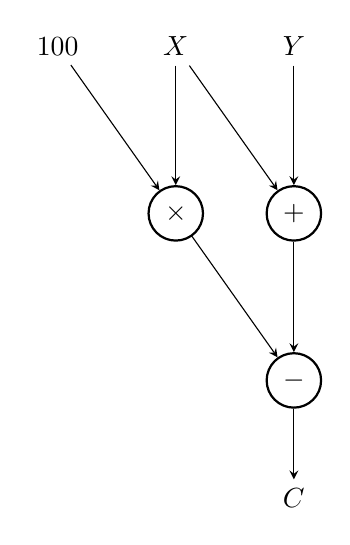
\begin{tikzpicture}[node distance={15mm}, main/.style = {draw, circle, thick}]
\node (100) {$100$};
\node (X)   [right of=100] {$X$};
\node (Y)    [right of=X] {$Y$};
\node[main] (plus) [below right of=X, below left of=Y] {$+$};
\node[main] (mul)  [below right of=100, below left of=X] {$\times$};
\node[main] (sub)  [below right of=mul, below left of=plus] {$-$};
\node (C)    [below of=sub] {$C$};

\draw[->, >=stealth] (100) -- (mul);
\draw[->, >=stealth] (X) -- (mul);
\draw[->, >=stealth] (X) -- (plus);
\draw[->, >=stealth] (Y) -- (plus);
\draw[->, >=stealth] (mul) -- (sub);
\draw[->, >=stealth] (plus) -- (sub);
\draw[->, >=stealth] (sub) -- (C);

\end{tikzpicture}
